%LaTex cheat sheet template
\documentclass[10pt,a4paper,landscape]{article}

\usepackage{xfrac}
\usepackage[utf8]{inputenc}
\usepackage{amsmath}
\usepackage{amsfonts}
\usepackage{amssymb}
\usepackage{multicol}
\usepackage{geometry}
\usepackage{lipsum}
\usepackage{titlesec}
\usepackage[nodisplayskipstretch]{setspace}
\usepackage{enumitem}
\usepackage{wrapfig}

\geometry{a4paper, left=0mm, top=0mm, right=0mm, bottom=1mm}

\titlespacing{\section}{0pt}{0pt}{0pt}
\titlespacing{\subsection}{0pt}{0pt}{0pt}
\titlespacing{\subsubsection}{0pt}{0pt}{0pt}

\setlength{\abovedisplayskip}{0pt}
\setlength{\belowdisplayskip}{0pt}
\setlength{\parindent}{0pt}

\begin{document}
\begin{multicols*}{4}
    \section*{Formulaire MachLe}
    \subsection*{Fundamentals}
\textbf{Definitions}

\underline{1:} A computer program is said to
learn from experience E with respect to some task T
and some performance measure P, if its performance
on T, as measured by P, improves with experience E.

\underline{2:} Set of computer methods that
analyse observation data to automatically detect
patterns, and then use the uncovered patterns to
perform functions on new un-observed data. Examples
of functions include : prediction, classification,
clustering and more generally decision making.

\textbf{Two main types:}

\underline{Supervised learning:} the goal is to learn a
mapping from inputs x to outputs y given a set of
example data called the training set.

\underline{Unsupervised learning:} the goal is to discover
interesting structures from inputs x given a set of data
called the training set.

A classification task maps inputs x to a finite set of
discrete outputs y. The outputs are the class labels
corresponding to the different categories we want to
predict. A regression task maps inputs x to an infinite set of
continuous outputs y. The outputs are numeric values
corresponding to the variable we want to predict.

    \subsection*{General ML methods}
\noindent
\textbf{Setting Hyperparameters:}

\underline{Idea 1:} Split the training set into a training set and a test set.

\underline{Idea 2:} Split the training set into a training set, a validation set and a test set.

\underline{Idea 3:} Split datas into folds try each folds as validation set and average the results.

\underline{Curse of dimensionality:} is when we observe a decrease of
performance when increasing the number of features. This is due to the
lack of samples N with respect to the dimensions D of the input space.

\textbf{Model evaluation:}

\underline{accuracy} $= \frac{TP + TN}{TP + TN + FP + FN}$.

\underline{precision} $= \frac{TP}{TP + FP}$.

\underline{recall} $= \frac{TP}{TP + FN}$.

\underline{F1 score} $= 2\cdot\frac{\text{precision}\cdot \text{recall}}{\text{precision} + \text{recall}}$

\textbf{Normalization:}

\underline{min-max rescaling} $= \frac{x - x_{min}}{x_{max} - x_{min}}$.
For strong outliners.

\underline{min-max normalization} $= 2\cdot \frac{x - x_{min}}{x_{max} - x_{min}}-1$.
For strong outliners.

\underline{z-norm} $= \frac{x - \mu}{\sigma}$.
For normal outliners.

\underline{log scaling} $= log(x)$.
For tail distribution.

\textbf{Encoding:}

\underline{1-hot:} association of 1 input for 1 category (ex 1 for cat, 0 for dog).

\underline{ordinal:} association of 1 input for 1 category (ex 1 for cat, 2 for dog).

\underline{word embedding:} projection of a word into a vector space.

\textbf{Learning curves:} plot of the training and validation error $J(\theta)$ as a
function of the number of training examples.

\underline{High bias:} underfitting, the model is too simple, getting more data won't help.
On the learning curve, the training and validation error are close and high.

\underline{High variance:} overfitting, the model is too complex, getting more data will help.
On the learning curve, the training error is low and the validation error is high.

\textbf{Dimensionality reduction:} transforms high-dimensional
data into a low-dimensional space, retaining meaningful properties of the original data.

\underline{Feature selection:} select only a few features are relevant to the task.

\underline{PCA:} uses orthogonal transformation to convert correlated variables into uncorrelated
"principal components". The first component maximizes variance, with each subsequent component
orthogonal to the previous, maximizing remaining variance.
Given a dataset $X$, create an $N\times d$ matrix, subtract the mean of each
vector $x_n$ in $X$, compute the covariance matrix, compute the eigenvectors and eigenvalues of
$\Sigma$, the $M$ eigenvectors with the highest eigenvalues are the principal components.

\underline{t-SNE:} t-distributed stochastic neighbor embedding, tries to group
local data points closer to each other. It uses a parameter called perplexity to
guess the number of close neighbors : $Perp(P_i)=2^{-\sum_{j}p_{j|i}\log_2p_{j|i}}$.
Tipically, perplexity is between 5 and 50. It is a non-linear dimensionality reduction.
It tipically uses PCA to reduce the dimensionality to 50 before applying t-SNE.

\underline{UMAP:} Uniform Manifold Approximation and Projection, faster than t-SNE,
allows to work with high dimensional data directly, uses the number of neighbors
instead of perplexity.
    \subsection*{K-NN}
k-nearest neighbour algorithm is a
method that classifies unlabelled examples based on
their similarity with examples in the training set.
It can be used for both classification and regression.

\textbf{Distance metric:}

\underline{L1 (Manhattan):} $d(I_1, I_2) = \sum_{i=1}^{n} |I_1^p - I_2^p|$

\underline{L2 (Euclidean):} $d(I_1, I_2) = \sqrt{\sum_{i=1}^{n} (I_1^p - I_2^p)^2}$

\textbf{Hyperparameters to tune:}

\underline{Normalization:} type : non, min-max, z-score.

\underline{distance metric:} L1, L2.

\underline{k:} number of neighbours.

K-NN is heavy to compute in terms of memory and CPU time. Memory : full training set needs to be stored.
CPU : the distance is computed against all training examples.

    \subsection*{Bayes}
$P(C_k|x) = \frac{P(x|C_k)P(C_k)}{P(x)}$

\underline{posteriori probability:} probability of class j given observation x

\underline{likelihood:} probability of observing x given class j

\underline{priori probability:} probability of class j

\underline{evidence:} probability of x unconditional to any class

\textbf{Multiple ways to estimate $P(x|C_k)$:}

\underline{Univariate Gaussian:}

$P(x|C_k) = \frac{1}{\sqrt{2\pi\sigma_{C_k}^2}}e^{\frac{-(x-\mu_{C_k})^2}{2\sigma_{C_k}^2}}$

\underline{Multivariate Gaussian (Naive Bayes):}

$P(x|C_k) = \frac{\prod_{i=1}^{D}}{\sqrt{2\pi\sigma_{C_k}^2}}e^{\frac{-(x_i-\mu_{C_k})^2}{2\sigma_{C_k}^2}}$

\underline{Univariate/multivariate Gaussian mixture:}
$P(x|C_k) = \sum_{i=1}^{K}\omega_{C_k}^{(i)}\mathcal{N}(x|\mu_{C_k}^{(i)}, \sigma_{C_k}^{(i)})$

with $\mu$ the mean, $\sigma$ the standard deviation, $\Sigma$ the covariance matrix,
$\omega$ the weight of the Gaussian, $K$ the number of Gaussians.

    \subsection*{Linear Regression}
The goal is to find the best mapping function : $\hat{y}=h_\theta(\overrightarrow{x})$, with $h_\theta(\overrightarrow{x})=\sum_{i=0}^{N}\theta_ix_i=\overrightarrow{\theta}^T\overrightarrow{x}$

\textbf{Cost function (MSE):}

$J(\theta)=\frac{1}{2N}\sum_{i=1}^{N}(h_\theta(\overrightarrow{x_i})-y_i)^2$

\textbf{Closed form solution:} usually too expensive to compute :

$\overrightarrow{\theta}=(X^TX)^{-1}X^T\overrightarrow{y}$

\textbf{Gradient descent:} minimize the cost function

\underline{Classic:} $\theta_i:=\theta_i-\alpha\frac{1}{N}\sum_{i=1}^{N}(h_\theta(\overrightarrow{x_i})-y_i)x_i$.
The learning rate $\alpha$ must be small enough to converge and large enough to converge in a reasonable time.

\underline{Stochastic gradient descent:} wich is faster but more noisy : $\theta_i:=\theta_i-\alpha(h_\theta(\overrightarrow{x_i})-y_i)x_i$.

\underline{Batched gradient descent} wich is faster but the batched size $b$ must
be optimized.

\underline{Stop condition:} $\frac{J(\theta)^{epoch_{n-1}}-J(\theta)^{epoch_{n}}}{J(\theta)^{epoch_{n}}}<\varepsilon$

If a dependency of $y$ with respect to $x$ is suspected to be non-linear :
$h_\theta(\overrightarrow{x})=\theta_0+\theta_1x_1+\theta_2x_1^2$
    \subsection*{Logistic Regression}
The logistic regression is an extension of the linear regression : $h_\theta(\overrightarrow{x})=g(\overrightarrow{\theta}^T\overrightarrow{x})$.
It is actually a one layer NN.

\textbf{Hypothesis function:} output 1 for a positive class and 0 for a negative class.

\underline{Sigmoid function:} $g(z)=\frac{1}{1+e^{-z}}$ and it's derivative : $g'(z)=g(z)(1-g(z))$.

\underline{Objective function:}

$J(\theta)=\frac{1}{N}\sum_{i=1}^{N}[y_i\log(h_\theta(\overrightarrow{x_i}))+(1-y_i)\log(1-h_\theta(\overrightarrow{x_i}))]$

\underline{Gradient:}

$\theta_i := \theta_i + \alpha\frac{1}{N}\sum_{i=1}^{N}(y_i-h_\theta(\overrightarrow{x_i}))x_i$.
    \subsection*{SVM}
\textbf{Linear SVM:} tries to find the hyperplane that separates the 2
classes and that maximizes the margin between the 2 classes.
SVM are particularly efficient for tasks with a high number of features and a low number of samples.

\underline{Hypothesis function:}

$h_w(\overrightarrow{x})=\text{sign}(b+\overrightarrow{w}^T\overrightarrow{x})$.

\underline{Margin:} distance between the hyperplane and the closest point of each class. Training samples
on the margin boundaries are called support vectors.

\underline{Hinge loss function:} used to calculate the slack :
$\xi_i=H(d(x_i, w, b))$, $d()$ is the distance from the boundary. That means
$\xi_i=0$ if $x_i$ is correctly classified and $\xi_i>0$ if $x_i$ is misclassified or
in the margin.

\underline{Loss function:} for two classes:

$J(w)=C[\frac{1}{N}\sum_{i=1}^{N}y_iH_{C1}(d(x_i, w, b))+(1-y_i)H_{C0}(d(x_i, w, b))]+\sfrac{\left\|w\right\|^2}{2}$.
The smaller the $C$, the greater the number of misclassified points.

\textbf{Kernel functions for non-linear problems:}
Compute a new test sample $x_t$ using a kernel funciton.

\underline{Linear:} $K(x_i, x_j)=x_ix_j$

\underline{Polynomial:} $K(x_i, x_j)=(x_ix_j+1)^d$

\underline{RBF:} $K(x_i, x_j)=\exp(-\gamma\left\|x_i-x_j\right\|^2)$

\underline{Hyperbolic tangent:}

$K(x_i, x_j)=\tanh(\kappa x_ix_j+\delta)$

\textbf{Multi-class classification:}

\underline{One-vs-all:} the SVM with the highest output value assigns the class to a sample.

\underline{One-vs-one:} each SVM assigns a sample to one of the two classes.
The class with the highest number of votes is assigned to the sample.






    \subsection*{K-MEANS}
K-Means is an unsupervised algorithm that finds clusters in the data. It is mathematically
guaranteed to converge but can converge to a local minimum.

\textbf{Terminology:}

\underline{Centroids:} the center of the clusters.

\underline{Codebook:} the set of centroids.

\underline{Partition:} the set of samples assigned to a centroid.

\textbf{Distortion function:}

$J(c, \mu)=\sum_{i=1}^{N} = d(x_n, \mu_{C_n})^2$.

$C_n$ is the centroid of the cluster to which $x_n$ is assigned.
$\mu_{C_n}$ is the centroid of the cluster $C_n$. $d()$ is the distance function and can
be the euclidean or manhattan distance.

\textbf{Elbow method:}
finds the optimal number of clusters. It plots the distortion
function vs the number of clusters. The number of clusters after which the distortion function
starts to decrease slowly is the optimal.


    \subsection*{Decision Trees}
Implements a sequence of decisions
on individual features allowing to classify the input data
at the end of the sequence. The decisions are taken
comparing a selected feature against a reference value.
The decisions are organised in a binary tree where each
decision split the input space into two branches.

\textbf{Gini impurity:}

\underline{Of a set:}

$G_{set} = 1 - \sum_{i=1}^{K} P(C_k)^2$ where
$P(C_k)=\sfrac{N_k}{N}$ measure how ofen a randomly chosen element
from the set would be incorrectly labeled if it was randomly labeled.
$N_k$ is the number of elements of class $k$ in the set.

\underline{Of a split:}

$G_{split} = \frac{N_{left}}{N}G_{left} + \frac{N_{right}}{N}G_{right}$.
is the weighted sum of the Gini impurity of the two sets after the split.
The weights are the proportions in the set.

\underline{Gain:} $G_{gain} = G_{set} - G_{split}$.

\textbf{Overfitting:}

\underline{Early stopping:} stop growing the tree after a certain depth.

\underline{Pruning:} grow a full tree and trim it afterwards.

\underline{Boosting:} build aditional trees on the weakneses of the previous ones.

\underline{Random Forest:} build multiple trees on random subsets of the data and average
their predictions.

\textbf{XGBoost} : (go-to solution) is a boosting algorithm that uses gradient boosting
to build the trees (implies the existence of a loss function).

    \subsection*{Neural Networks}
A neural network is a set of neurons connected together. Each neuron is a function
that takes a vector as input and outputs a scalar. The output of a neuron is
computed as follows : $y = f(\sum_{i=1}^{N} w_i x_i + b)$ where $w_i$ are the weights,
$x_i$ are the inputs, $b$ is the bias and $f$ is the activation function.

\textbf{Forward propagation:}

Instead of beeing constrained by its own features
$\overrightarrow{x}$, the neural network gets to learn its own features
to feed into the logistic regression.

\textbf{Cost function:}

$J(\Theta)=-\frac{1}{m}[\sum_{i=1}^{m}\sum_{k=1}^{K}y_k^{(i)}\log(h_\Theta(x^{(i)}))_k+(1-y_k^{(i)})\log(1-(h_\theta(x^{(i)}))_k)]+\frac{\lambda}{2m}\sum_{l=1}^{L-1}\sum_{i=1}^{s_l}\sum_{j=1}^{s_{l+1}}(\Theta_{ji}^{(l)})^2$

$^{(i)}$ is the layer number. $s_l$ is the number of units in layer $l$. $\lambda$ is the regularization parameter. $L$ is the total number of layers. $K$ is the number of output units.
Neural network's cost function extends logistic regression's to handle multiple outputs.

\textbf{Backpropagation:}

The equivalent of gradient descent for neural networks.
It is used to compute the partial derivatives $\frac{\partial}{\partial\Theta_{ij}^{(l)}}J(\Theta)$.
There is also back propagation with momentum to avoid local minima.

\textbf{Activation functions} :

\underline{sigmoid} : $g(z)=\frac{1}{1+e^{-z}}$

\underline{tanh} : $g(z)=\frac{e^z-e^{-z}}{e^z+e^{-z}}$

\underline{ReLU} : $g(z)=\max(0,z)$

\underline{Linear} : $g(z)=z$
    \subsection*{Convolutional Neural Networks}
Convolutional Neural Networks (CNNs) process spatial data using
convolutions, extracting diverse features from images with multiple
filters. They detect hierarchical features by linking filter layers,
and use new activation functions to mitigate vanishing gradients.
CNNs summarize lower layer feature statistics via down-sampling and
employ techniques like dropout to prevent overfitting.

Each hidden neuron process a small region of the image. Different kernel sizes
allows the identification of features at different scales. Zeros padding allows
the output to have the same size as the input.

Multiple convolutions look for different features. The output of a convolutional
layer with 30 kernels gives 30 images.

Sigmoid activation functions can cause vanishing gradients due to their derivatives
nearing zero. Softmax in the output layer calculates a categorical
probability distribution : $f(x_i)=\sfrac{e^{x_i}}{\sum_{j=1}^{K}e^{x_j}}$.

Maxpooling after convolution reduces computation by down-sampling non-maximal
values, summarizing lower layer feature statistics. It results in smaller images.

The resulting architecture of a CNN is a stack of alternating convolutional and
pooling layers, followed by a fully connected layer.

Dropout in CNNs randomly deactivates neurons during training to prevent
overfitting, enhancing model generalization by reducing complex
co-dependencies on training data.
    \subsection*{Recurrent Neural Networks}
Memorize previous output or hidden layer to feed it back in the network in the next iteration.
\setlength{\intextsep}{-5pt}
\begin{wrapfigure}{l}{0.05\textwidth}
    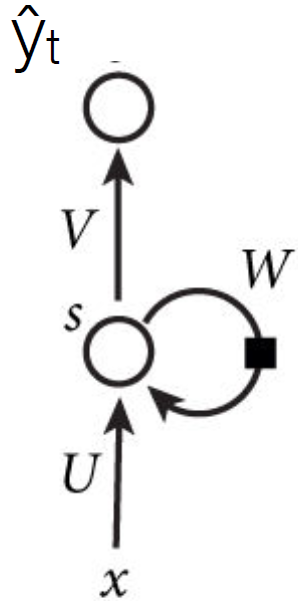
\includegraphics[width=\linewidth]{images/BPTT.png}
\end{wrapfigure}
We sum errors across a sequence of correct outputs $y_t$ and predicted ones
$\hat{y}_t$, treating the sequence as one training example.
$s_t=\text{tanh}(Ux_t+Ws_{t-1})$\\
$\hat{y}_t=\text{softmax}(Vs_t)$\\
$E(y,\hat{y})=-\sum_{t}y_t\log\hat{y}_t$\\
$\frac{\partial E}{\partial W}=\sum_{t}\frac{\partial E_t}{\partial W}$
thus, in general, the larger the temporal horizon, the longer the chain rule of derivatives.
Gradients from distant steps become zero, hindering learning of long-range dependencies.
Modern RNNs use LSTM (Long Short-Term Memory) cells to mitigate this problem.
LSTM cells have a memory cell $c_t$ and three gates: input $i_t$, forget $f_t$ and output $o_t$.
    \subsection*{Reinforcement Learning}
Learns from interaction with an environment, optimizing a reward function.
RL problems can be modeled as Markov Decision Processes (MDPs), which consist of a set
of states, a set of actions, a transition function, and a reward function. The goal
of RL is to find a policy that maps states to actions, and maximizes the expected return,
which is the discounted sum of future rewards.

\textbf{Value functions:} estimate the expected return from a given state or
state-action pair. Value functions can be learned by dynamic programming,
\textit{Monte Carlo} or \textit{temporal-difference learning}.

\textbf{Value-based methods (SARSA):} learn a value function and derive a policy from it.

\textbf{Policy-based methods:} methods that learn a policy directly, without using a value function.

\textbf{Exploration-exploitation trade-off:} the dilemma of choosing between actions
that have high expected reward (exploitation) and actions that have high
uncertainty (exploration).

\underline{$\varepsilon$-greedy:} with probability $\varepsilon$, choose a random action, otherwise choose the best action.

\underline{Boltzmann:} $P(a|s)=\frac{e^{\frac{Q(s, a)}{\tau}}}{\sum_{b\in a}e^{\frac{Q(s, b)}{\tau}}}$
Explore based on the probability of each action.


\end{multicols*}
\end{document}